\documentclass[titlepage]{article}
\usepackage{babel}
\usepackage{amsmath}
\usepackage{amssymb}
\usepackage{amsthm}
\usepackage{multicol} %spalten in seite
\usepackage{graphicx} %bilder einfügen
\usepackage{tabto} %tabulator mit \tab
\usepackage{hyperref}
\usepackage[T1]{fontenc}
\usepackage{mathrsfs}  
\usepackage[utf8]{inputenc}
\usepackage{listings} %quellcode
\pagestyle{plain}
\usepackage{xcolor}
\pagenumbering{arabic}
\renewcommand{\arraystretch}{1.3} %vertikaler abstand von tabellen
\newcommand{\n}{\newline}
\usepackage[left=20mm, right=15mm, top=25mm, bottom=30mm, paper=a4paper]{geometry}

\usepackage{pgfplots}
\pgfplotsset{compat=1.15}
\usepackage{mathrsfs}
\usetikzlibrary{arrows}

\begin{document}
	
	\title{Diskrete Strukturen - Übung 03}
	\author{Felix Tischler, Martrikelnummer: 191498}
	\date{\today}
	\maketitle
	
	\section*{1.) Der Turm von Hanoi}
		\subsection*{a)}
		Sei T(n) die kleinstmögliche Anzahl von Zugfolgen. Für kleine Werte von n folgt:
		\begin{table}[h]
			\begin{tabular}{c|ccc}
				n&1&2&3\\\hline
				T(n)&2&8&26
			\end{tabular}
		\quad
			\begin{tabular}{c|c}
				T(1)&2\\\hline
				T(2)&3 T(1)+2 = 8\\\hline
				T(3)&3 T(2)+2 = 26\\
			\end{tabular}
		\quad$\Rightarrow$\quad
			\begin{tabular}{lrl}
				a)& T(1) &= 2\\
				b)& T(n+1) &= 3 T(n) + 2
			\end{tabular}
		\end{table}
	
		\noindent
		Wenn wir nun mit dieser Formel einige weitere Werte für n > 1 berechnen folgt:
		\begin{table}[h]
			\begin{tabular}{c|cccc}
				n&2&3&4&5\\\hline
				T(n)&\textcolor{blue}{8}&\textcolor{blue}{26}&\textcolor{blue}{80}&\textcolor{blue}{242}\\
				$2^n$&4&8&16&32\\
				$3^n$&9&27&81&243\\
				$3^n-1$&\textcolor{blue}{8}&\textcolor{blue}{26}&\textcolor{blue}{80}&\textcolor{blue}{242}
			\end{tabular}
		\quad$\Rightarrow$\quad
			\begin{tabular}{c}
				$\forall n \in\mathbb{N}\textbackslash\{0,1\}$: T(n) = $3^n-1$
			\end{tabular}
		\end{table}
	
		\noindent
		Nun gilt es mithilfe von a), b) dies zu beweisen.
		
		\subsubsection*{Induktionsanfang}
		\begin{tabular}{lccl}
			$T(2)$ & $=$ & $3^2-1$ & \\
			& $=$ & $8$ &
		\end{tabular}
		
		\subsubsection*{Induktionsvoraussetzung IV}
		für $n=k \in \mathbb{N},\,k > 1 \, :$
		\begin{tabular}{lcc}
			$T(k)$ & $=$ & $3^k-1$ \\
		\end{tabular}
	
		\subsubsection*{Induktionsbehauptung}
		für $n=k+1 : T(k+1)=3^{k+1}-1$
		
		\subsubsection*{Induktionsbeweis}
		\begin{align*}
			T(k+1) &\overset{c)}{=}3\cdot T(k)+2&&&&&&&&\\
			&\overset{IV}{=}3\cdot(3^k-1)+2\\	
			&=3^{k+1}-3+2\\
			&=3^{k+1}-1\qed				
		\end{align*}
	
		\subsection*{b)}
		Zuerst ist zu klären wie viele Möglichkeiten es überhaupt gibt. Dies sind genau $3^n$, da es insgesamt 3 Stapel, bzw. grundlegende Positionen gibt und insgesamt n verschiedene Elemente welche auf 3 Stapel verteilt werden. Dies sei kurz gezeigt am Beispiel für n=1 und n=2:
		\begin{table}[h]
			\begin{tabular}{c|ccccccccc}
				n&&&&&&&&&\\
				1&L&M&R&&&&&&\\
				2&LL&MM&RR&LM&ML&LR&RL&MR&RM
			\end{tabular}
		\end{table}
	
		\noindent
		Hierzu sein L, M, R die drei verschiedenen Stapel und sobald ein Buchstabe in der Tabelle erwähnt wird befindet sich eine Scheibe auf ihm. Z.B. AA symbolisiert dass 2 Scheiben auf A liegen. AA darf des weiteren nur einmal vorkommen da (H2) gilt. Man benötigt also effektiv $3^n-1$ Züge um alle Möglichkeiten durchzugehen, da ja immer mindestens eine Möglichkeit erfüllt ist ohne einen Zug zu verbrauchen und zwar genau die Startposition. Da es im Spiel keine doppelten Züge geben kann (wenn man von der kürzesten Schrittfolge ausgeht) ist nun nur zu Zeigen, dass es immer mindestens $3^n-1$ Spielzüge gibt, damit alle Möglichkeiten abgedeckt werden. Dieser Beweis wurde bereits in der Teilaufgabe a) vollzogen. Somit ist bewiesen, dass alle Möglichkeiten abgedeckt sind.
	\section*{2.) Fibonacci-Zahlen}
	Im folgenden sehen sie ein Schema für die Visualisierung für die Fälle n = 1, 2, 3, 4, 5, 6, 7, anhand einer Schemazeichnung, wobei ein Blauer Punkt eine Drohne symbolisiert und ein Brauner Punkt eine Königin:\\\\
		\definecolor{ududff}{rgb}{0.30196078431372547,0.30196078431372547,1}
		\definecolor{ccqqqq}{rgb}{0.8,0,0}
		\begin{tikzpicture}[line cap=round,line join=round,>=triangle 45,x=1cm,y=1cm]
			\clip(-13.666331645622149,-5.0028147095331) rectangle (14.301361081252827,8.616868988189845);
			\draw [line width=2pt] (-12,1)-- (-11,1);
			\draw [line width=2pt] (-11,1)-- (-8,2);
			\draw [line width=2pt] (-11,1)-- (-8,1);
			\draw [line width=2pt] (-8,2)-- (-5,2);
			\draw [line width=2pt] (-8,2)-- (-5,1);
			\draw [line width=2pt] (-5,2)-- (-2,4);
			\draw [line width=2pt] (-5,2)-- (-2,3);
			\draw [line width=2pt] (-2,4)-- (1,5);
			\draw [line width=2pt] (-2,4)-- (1,4);
			\draw [line width=2pt] (1,5)-- (4,8);
			\draw [line width=2pt] (1,5)-- (4,7);
			\draw [line width=2pt] (-8,1)-- (-5,0);
			\draw [line width=2pt] (-5,0)-- (-2,1);
			\draw [line width=2pt] (-5,0)-- (-2,0);
			\draw [line width=2pt] (-5,1)-- (-2,2);
			\draw [line width=2pt] (-2,3)-- (1,3);
			\draw [line width=2pt] (-2,2)-- (1,2);
			\draw [line width=2pt] (-2,2)-- (1,1);
			\draw [line width=2pt] (-2,1)-- (1,0);
			\draw [line width=2pt] (-2,1)-- (1,-1);
			\draw [line width=2pt] (-2,0)-- (1,-2);
			\draw [line width=2pt] (1,4)-- (4,6);
			\draw [line width=2pt] (1,3)-- (4,5);
			\draw [line width=2pt] (1,3)-- (4,4);
			\draw [line width=2pt] (1,2)-- (4,3);
			\draw [line width=2pt] (1,2)-- (4,2);
			\draw [line width=2pt] (1,1)-- (4,1);
			\draw [line width=2pt] (1,0)-- (4,0);
			\draw [line width=2pt] (1,0)-- (4,-1);
			\draw [line width=2pt] (1,-1)-- (4,-2);
			\draw [line width=2pt] (1,-2)-- (4,-3);
			\draw [line width=2pt] (1,-2)-- (4,-4);
			\begin{scriptsize}
				\draw [fill=ccqqqq] (-11,1) circle (2.5pt);
				\draw [fill=ududff] (-8,1) circle (2.5pt);
				\draw [fill=ccqqqq] (-8,2) circle (2.5pt);
				\draw [fill=ccqqqq] (-5,0) circle (2.5pt);
				\draw [fill=ududff] (-5,1) circle (2.5pt);
				\draw [fill=ccqqqq] (-5,2) circle (2.5pt);
				\draw [fill=ududff] (-2,3) circle (2.5pt);
				\draw [fill=ccqqqq] (-2,4) circle (2.5pt);
				\draw [fill=ccqqqq] (-2,2) circle (2.5pt);
				\draw [fill=ccqqqq] (-2,1) circle (2.5pt);
				\draw [fill=ududff] (-2,0) circle (2.5pt);
				\draw [fill=ududff] (1,4) circle (2.5pt);
				\draw [fill=ccqqqq] (1,3) circle (2.5pt);
				\draw [fill=ccqqqq] (1,2) circle (2.5pt);
				\draw [fill=ududff] (1,1) circle (2.5pt);
				\draw [fill=ccqqqq] (1,0) circle (2.5pt);
				\draw [fill=ududff] (1,-1) circle (2.5pt);
				\draw [fill=ccqqqq] (1,5) circle (2.5pt);
				\draw [fill=ccqqqq] (1,-2) circle (2.5pt);
				\draw [fill=ccqqqq] (4,6) circle (2.5pt);
				\draw [fill=ccqqqq] (4,5) circle (2.5pt);
				\draw [fill=ududff] (4,4) circle (2.5pt);
				\draw [fill=ccqqqq] (4,3) circle (2.5pt);
				\draw [fill=ududff] (4,2) circle (2.5pt);
				\draw [fill=ccqqqq] (4,1) circle (2.5pt);
				\draw [fill=ccqqqq] (4,0) circle (2.5pt);
				\draw [fill=ududff] (4,-1) circle (2.5pt);
				\draw [fill=ccqqqq] (4,-2) circle (2.5pt);
				\draw [fill=ccqqqq] (4,-3) circle (2.5pt);
				\draw [fill=ududff] (4,-4) circle (2.5pt);
				\draw [fill=ududff] (4,7) circle (2.5pt);
				\draw [fill=ccqqqq] (4,8) circle (2.5pt);
				\draw [fill=ududff] (-12,1) circle (2.5pt);
			\end{scriptsize}
		\end{tikzpicture}
	Zu beachten ist, dass dieser Stammbaum der Drohne fortlaufend die vorherigen Generationen zeigt. So sieht man zunächst eine Drohne (Blauer Punkt), dann eine Königin (Brauner Punkt) als Elternteil, und dann wiederum eine Königin und eine Drohne als Eltern der Königin. Und so weiter... Es ist die Fibonacci Folge zu erkennen wenn man immer alle existierenden Punkte der jeweiligen Stufe betrachtet. Denn sie bestehen immer aus den 2 vorherigen Stufen. Somit gibt es für eine Drohne in der 1. Vorfahrensgeneration genau 1 Vorfahren und zwar die Königin. Sei nun n die Vorfahrensgeneration und f(n) die Anzahl der Vorfahren der aktuellen Generation. So gilt:
	\begin{align*}
		f(1)&=1\\
		f(n+1)&=f(n)+f(n-1)
	\end{align*}

	\newpage
	\noindent
	Im folgenden wird dieser Zusammenhang mathematisch hergeleitet.
	
	\begin{table}[h]
		\begin{tabular}{rl}
			$K(n)$&...Anzahl der Königin in der n-ten Generation.\\
			$D(n)$&...Anzahl der Drohnen in der n-ten Generation.\\
			$V(n)$&...Anzahl der gesamten Vorfahren in der n-ten Generation.\\
		\end{tabular}
	\end{table}

	\noindent
	Folgende Zusammenhänge fallen bei genauerer Betrachtung des Schemas auf:
	\begin{align*}
		V(n)&=K(n)+D(n)\\
		K(n)&=V(n-1)\\
		D(n)&=K(n-1)\\
		V(n)&=V(n-1)+K(n-1)
	\end{align*}
	
	\noindent
	Nun ist $V(n+1)=V(n)+V(n-1)$ zu zeigen.
	\begin{align*}
			V(n+1)&=V(n)+K(n)\\
			&=V(n)+V(n-1)\qed
	\end{align*}

	\section*{3.) Fibonacci-Zahlen}
		Mit $f_n=\frac{\Phi^n-\Psi^n}{\Phi-\Psi}$, $\Phi^{-1}=-\Psi$, $\Psi^{-1}=-\Phi$, $\Phi=\frac{1+\sqrt{5}}{2}$ und $\Psi=\frac{1-\sqrt{5}}{2}$ folgt:
		\begin{align*}
			\frac{\Phi^{2n}-\Psi^{2n}}{\sqrt{5}}&=\frac{\Phi^{n}-\Psi^{n}}{\sqrt{5}}\cdot\left(\frac{\Phi^{n+1}-\Psi^{n+1}}{\sqrt{5}}+\frac{\Phi^{n-1}-\Psi^{n-1}}{\sqrt{5}}\right)\\
			&\overset{Distr.}{\Leftrightarrow}\frac{\Phi^{n}-\Psi^{n}}{\sqrt{5}}\cdot\frac{\Phi^{n+1}-\Psi^{n+1}}{\sqrt{5}} +\frac{\Phi^{n}-\Psi^{n}}{\sqrt{5}}\cdot\frac{\Phi^{n-1}-\Psi^{n-1}}{\sqrt{5}}\\
			&\Leftrightarrow\frac{1}{5}\cdot(\Phi^n\cdot\Phi^{n+1}-\Phi^n\cdot\Psi^{n+1}-\Psi^n\cdot\Phi^{n+1}+\Psi^n\cdot\Psi^{n+1}+\Phi^n\cdot\Phi^{n-1}-\Phi^n\cdot\Psi^{n-1}-\Psi^n\cdot\Phi^{n-1}+\Psi^n\cdot\Psi^{n-1})\\
			&\Leftrightarrow\frac{1}{5}\cdot(\Phi^{2n+1}-\Phi^n\cdot\Psi^{n+1}-\Psi^n\cdot\Phi^{n+1}+\Psi^{2n+1}+\Phi^{2n-1}-\Phi^n\cdot\Psi^{n-1}-\Psi^n\cdot\Phi^{n-1}+\Psi^{2n-1})\\
			&\Leftrightarrow\frac{1}{5}\cdot(\Phi^{2n+1}+\Phi^{2n-1}+\Psi^{2n+1}+\Psi^{2n-1}-\Phi^n\cdot\Psi^{n+1}-\Phi^n\cdot\Psi^{n-1}-\Psi^n\cdot\Phi^{n+1}-\Psi^n\cdot\Phi^{n-1})\\
			&\overset{Distr.}{\Leftrightarrow}\frac{1}{5}\cdot(\Phi^{2n}\cdot(\Phi+\Phi^{-1})+\Psi^{2n}\cdot(\Psi+\Psi^{-1})+\Phi^n\cdot(-\Psi^{n+1}-\Psi^{n-1})+\Psi^n\cdot(-\Phi^{n+1}-\Phi^{n-1}))\\
			&\overset{Distr.}{\Leftrightarrow}\frac{1}{5}\cdot(\Phi^{2n}\cdot(\Phi+\Phi^{-1})+\Psi^{2n}\cdot(\Psi+\Psi^{-1})+\Phi^n\cdot\Psi^n\cdot(-\Psi-\Psi^{-1})+\Psi^n\cdot\Phi^n\cdot(-\Phi-\Phi^{-1}))\\	
			&\Leftrightarrow\frac{1}{5}\cdot(\Phi^{2n}\cdot(\Phi-\Psi)+\Psi^{2n}\cdot(\Psi-\Phi)+\Phi^n\cdot\Psi^n\cdot(-\Psi+\Phi)+\Psi^n\cdot\Phi^n\cdot(-\Phi+\Psi))\\
			&\overset{Distr.}{\Leftrightarrow}\frac{1}{5}\cdot(\Phi^{2n}\cdot(\Phi-\Psi)+\Psi^{2n}\cdot(\Psi-\Phi)+\Phi^n\cdot\Psi^n\cdot(-\Psi+\Phi-\Phi+\Psi))\\
			&\Leftrightarrow\frac{1}{5}\cdot(\Phi^{2n}\cdot(\Phi-\Psi)+\Psi^{2n}\cdot(\Psi-\Phi)=\frac{1}{5}\cdot(\Phi^{2n}\cdot\left(\frac{1+\sqrt{5}}{2}-\frac{1-\sqrt{5}}{2}\right)+\Psi^{2n}\cdot\left(\frac{1-\sqrt{5}}{2}-\frac{1+\sqrt{5}}{2}\right)\\
			&\Leftrightarrow\frac{1}{5}\cdot(\Phi^{2n}\cdot\sqrt{5}-\Psi^{2n}\cdot\sqrt{5})=\frac{\Phi^{2n}\cdot\sqrt{5}-\Psi^{2n}\cdot\sqrt{5}}{\sqrt{5}\cdot\sqrt{5}}=\frac{\Phi^{2n}-\Psi^{2n}}{\sqrt{5}}\qed
		\end{align*}
	\newpage
	\section*{4.) Goldener Schnitt}
	\subsection*{a)}
	Im folgenden ist die Strecke AB zu sehen, welche im Punkt T geschnitten wird und somit in eine kleinere Strecke l und eine größere Strecke G geteilt wird. Dies ist nicht wie in Aufgabe 2 erwartet eine gültige Konstruktion. Es ist eine Visualisierung welche als Grundlage meiner Argumentation zu betrachten ist.
	
	\definecolor{xdxdff}{rgb}{0.49019607843137253,0.49019607843137253,1}
	\definecolor{uuuuuu}{rgb}{0.26666666666666666,0.26666666666666666,0.26666666666666666}
	\begin{tikzpicture}[line cap=round,line join=round,>=triangle 45,x=1cm,y=1cm]
		\clip(-0.9758674155848819,-1.5846081100011586) rectangle (12.283896684789129,1.667540721229959);
		\draw [line width=2pt] (0,0)-- (1.7900072659769493,0);
		\draw [line width=2pt] (1.7900072659769493,0)-- (5,0);
		\begin{scriptsize}
			\draw [fill=uuuuuu] (0,0) circle (2pt);
			\draw[color=uuuuuu] (0.10025149927756115,0.23984637209321286) node {$A$};
			\draw [fill=xdxdff] (5,0) circle (2.5pt);
			\draw[color=xdxdff] (5.097401402776723,0.26458473795211956) node {$B$};
			\draw [fill=xdxdff] (1.7900072659769493,0) circle (2.5pt);
			\draw[color=xdxdff] (1.8937830240482996,0.26458473795211956) node {$T$};
			\draw[color=black] (0.9413559384803902,-0.24464483528421459) node {$l$};
			\draw[color=black] (3.4399308902299706,-0.24464483528421459) node {$L$};
		\end{scriptsize}
	\end{tikzpicture}

	Nun ist zu zeigen dass folgendes gilt:
	\begin{align*}
		\frac{L}{l}&=\frac{L+l}{L}\Rightarrow \frac{TB}{AT}=\frac{AB}{TB}
	\end{align*}

	Hierzu sei die Strecke AB = x und AT = 1, daraus ergeben sich folgende Zusammenhänge:
	\begin{align*}
		AB&=x\\
		AT&=1\\
		TB&=x-1
	\end{align*}
	
	Und somit folgt:
	\begin{align*}
		\frac{x-1}{1}&=\frac{x}{x-1}\\
		\Rightarrow x_{1,2}&=\frac{\pm\sqrt{5}+3}{2}\overset{Nur\,pos.}{\Rightarrow}=x=\frac{\sqrt{5}+3}{2}
	\end{align*}

	Dies nun eingesetzt in $x-1$, da ja $\frac{x-1}{1}=\frac{x}{x-1}$ dem goldenen Schnitt entsprechen soll:
	\begin{align*}
			\frac{\sqrt{5}+3}{2}-1&\Rightarrow\frac{\sqrt{5}+1}{2}\qed
	\end{align*}

	\subsection*{b)}
	\definecolor{ududff}{rgb}{0.30196078431372547,0.30196078431372547,1}
	\begin{tikzpicture}[line cap=round,line join=round,>=triangle 45,x=1cm,y=1cm]
		\clip(-1.24156226394636263,-0.42773193500256884) rectangle (1.883337876537244,0.414296385645171);
		\draw [line width=2pt] (0,0)-- (1,0);
		\draw [line width=2pt] (1,0)-- (1.618033988749895,0);
		\begin{scriptsize}
			\draw [fill=ududff] (0,0) circle (2.5pt);
			\draw[color=ududff] (0.02520313784193754,0.30533445369603168) node {$A$};
			\draw [fill=ududff] (1.618033988749895,0) circle (2.5pt);
			\draw[color=ududff] (1.640782368896924,0.30533445369603168) node {$B$};
			\draw [fill=ududff] (1,0) circle (2.5pt);
			\draw[color=ududff] (1.0233253714992854,0.30533445369603168) node {$T$};
			\draw[color=black] (0.5107761163779446,-0.212597011994932537) node {$L$};
			\draw[color=black] (1.3200644139379563,-0.212597011994932537) node {$l$};
		\end{scriptsize}
	\end{tikzpicture}\footnote{T teilt exakt im goldenen SChnitt}\\

	Mit der in a) bewiesenen Gleichung wird nun für die Konstruktion folgendes vorausgesetzt:
	\begin{align*}
		\frac{L}{l}=\frac{\sqrt{5}+1}{2}
	\end{align*}

	Sei nun L = 1, dann folgt:
	\begin{align*}
		\frac{L}{l}&=\frac{\sqrt{5}+1}{2}\\
		\Rightarrow l&=\frac{\sqrt{5}-1}{2}
	\end{align*}

	Somit wird nun eine Strecke konstruiert, für die gilt:
	\begin{align*}
		L+l&=AB=1+\frac{\sqrt{5}-1}{2}\\
		L&=AT=1\\
		l&=TB=\frac{\sqrt{5}-1}{2}
	\end{align*}
	
	\subsection*{c)}
	
	Das folgende Rechteck wurde auf Grundlage der vorherigen Aufgabe und mit folgenden Maßen Konstruiert:
	\begin{table}[h]
		\begin{tabular}{ccccccc}
			$\overline{AA'}$&=&$\overline{TT'}$&=&$L$&=&$1$\\
			$\overline{AT}$&=&$\overline{A'T'}$&=&$l$&=&$\frac{\sqrt{5}-1}{2}$
		\end{tabular}
	\end{table}

	\definecolor{ududff}{rgb}{0.30196078431372547,0.30196078431372547,1}
	\begin{tikzpicture}[myscale/.style={scale=#1},myscale=10, line cap=round,line join=round,>=triangle 45,x=1cm,y=1cm]
		\clip(-0.24156226394636263,-0.42773193500256884) rectangle (3.283337876537244,0.704296385645171);
		\draw [line width=2pt] (0,0)-- (1,0);
		\draw [line width=2pt] (0,0.6180339887498949)-- (0,0);
		\draw [line width=2pt] (1,0.6180339887498949)-- (1,0);
		\draw [line width=2pt] (0,0.6180339887498949)-- (1,0.6180339887498949);
		\begin{scriptsize}
			\draw [fill=ududff] (0,0) circle (0.25pt);
			\draw[color=ududff] (0.02520313784193754,0.06533445369603168) node {\large$A$};
			\draw [fill=ududff] (1,0) circle (0.25pt);
			\draw[color=ududff] (1.0233253714992854,0.06533445369603168) node {\large$T$};
			\draw[color=black] (0.5107761163779446,-0.032597011994932537) node {\large$L$};
			\draw [fill=ududff] (1,0.6180339887498949) circle (0.25pt);
			\draw[color=ududff] (1.0353148277594337,0.6827914510936712) node {\large$T'$};
			\draw [fill=ududff] (0,0.6180339887498949) circle (0.25pt);
			\draw[color=ududff] (0.03719259410208586,0.6827914510936712) node {\large$A'$};
			\draw[color=black] (0.9633780901985438,0.34408931174448065) node {\large$l$};
		\end{scriptsize}
	\end{tikzpicture}
	
	
	\subsection*{d)}
	$\overline{A'A}=\overline{A'P}$
	
	\definecolor{ududff}{rgb}{0.30196078431372547,0.30196078431372547,1}
	\begin{tikzpicture}[myscale/.style={scale=#1, node distance=#1*10em},myscale=6.5, line cap=round,line join=round,>=triangle 45,x=1cm,y=1cm]
		\clip(-0.24156226394636263,-0.42773193500256884) rectangle (3.283337876537244,0.704296385645171);
		\draw [line width=2pt] (0,0)-- (1,0);
		\draw [line width=2pt] (0,0.6180339887498949)-- (0,0);
		\draw [line width=2pt] (1,0.6180339887498949)-- (1,0);
		\draw [line width=2pt] (0,0.6180339887498949)-- (1,0.6180339887498949);
		\draw [line width=2pt] (0.6180339887498949,0.6180339887498949)-- (0.6180339887498949,0);
		\begin{scriptsize}
			\draw [fill=ududff] (0,0) circle (0.25pt);
			\draw[color=ududff] (0.02520313784193754,0.06533445369603168) node {\large$A$};
			\draw [fill=ududff] (1,0) circle (0.25pt);
			\draw[color=ududff] (1.0533253714992854,0.06533445369603168) node {\large$T$};
			\draw [fill=ududff] (1,0.6180339887498949) circle (0.25pt);
			\draw[color=ududff] (1.0353148277594337,0.6827914510936712) node {\large$T'$};
			\draw [fill=ududff] (0,0.6180339887498949) circle (0.25pt);
			\draw[color=ududff] (0.03719259410208586,0.6827914510936712) node {\large$A'$};
			\draw [fill=ududff] (0.6180339887498949,0) circle (0.25pt);
			\draw[color=ududff] (0.7505968728004661,0.06533445369603168) node {\large$Teilung$};
			\draw [fill=ududff] (0.6180339887498949,0.6180339887498949) circle (0.25pt);
			\draw[color=ududff] (0.6426601352395762,0.6827914510936712) node {\large$P$};
		\end{scriptsize}
	\end{tikzpicture}
	
	\newpage
	 Für jede weitere Teilung werden immer 2 Kreise verwendet die als Radius immer $l$ haben. Wobei es sich um das aktuelle $l$ handelt, welches bei jeder Teilung neu definiert wird. Der exakte Wert ist dabei uninteressant, da es am Anfang gegeben. Somit kann jede weiter Teilung über die Verwendung von 2 Kreisen erfolgen. Dazu werden die Kreise gezeichnet wie in den folgenden 2 Abbildungen und jeweils die Schnittpunkte mit den Geraden begrenzen das neue Quadrat. In den nächsten Abbildungen wird auf die Kreise verzichtet in der Visualisierung damit es übersichtlich bleibt, jedoch sei erwähnt das mit ihnen jedes weitere Quadrat konstruiert wurde.\\\\
	 $\overline{PT'}=\overline{T'Teilung}$,
	
	\definecolor{uuuuuu}{rgb}{0.26666666666666666,0.26666666666666666,0.26666666666666666}
	\definecolor{ududff}{rgb}{0.30196078431372547,0.30196078431372547,1}
	\begin{tikzpicture}[myscale/.style={scale=#1, node distance=#1*10em},myscale=6.7, line cap=round,line join=round,>=triangle 45,x=1cm,y=1cm]
		\clip(-0.24156226394636263,-0.42773193500256884) rectangle (3.283337876537244,1.1204296385645171);
		\draw [line width=2pt] (0,0.6180339887498949)-- (0,0);
		\draw [line width=2pt] (1,0.6180339887498949)-- (1,0);
		\draw [line width=2pt] (0,0.6180339887498949)-- (1,0.6180339887498949);
		\draw [line width=2pt] (0.6180339887498949,0.6180339887498949)-- (0.6180339887498949,0);
		\draw [line width=2pt] (0.6180339887498949,0)-- (1,0);
		\draw [line width=2pt] (0.6180339887498949,0)-- (0,0);
		\draw [line width=2pt] (1,0.6180339887498949) circle (0.3819660112501051cm);
		\begin{scriptsize}
			\draw [fill=ududff] (0,0) circle (0.25pt);
			\draw [fill=ududff] (1,0) circle (0.25pt);
			\draw [fill=ududff] (1,0.6180339887498949) circle (0.25pt);
			\draw[color=ududff] (1.0353148277594337,0.6827914510936712) node {\large$T'$};
			\draw [fill=ududff] (0,0.6180339887498949) circle (0.25pt);
			\draw [fill=ududff] (0.6180339887498949,0) circle (0.25pt);
			\draw [fill=ududff] (0.6180339887498949,0.6180339887498949) circle (0.25pt);
			\draw[color=ududff] (0.6426601352395762,0.6827914510936712) node {\large$P$};
			\draw [fill=uuuuuu] (1,0.23606797749978983) circle (0.25pt);
			\draw[color=uuuuuu] (1.0823253714992854,0.2931341226388502) node {\large$Teilung$};
		\end{scriptsize}
	\end{tikzpicture}

	\definecolor{uuuuuu}{rgb}{0.26666666666666666,0.26666666666666666,0.26666666666666666}
	\definecolor{ududff}{rgb}{0.30196078431372547,0.30196078431372547,1}
	\begin{tikzpicture}[myscale/.style={scale=#1, node distance=#1*10em},myscale=6.7, line cap=round,line join=round,>=triangle 45,x=1cm,y=1cm]
		\clip(-0.24156226394636263,-0.42773193500256884) rectangle (3.283337876537244,1.104296385645171);
		\draw [line width=2pt] (0,0.6180339887498949)-- (0,0);
		\draw [line width=2pt] (1,0.6180339887498949)-- (1,0);
		\draw [line width=2pt] (0,0.6180339887498949)-- (1,0.6180339887498949);
		\draw [line width=2pt] (0.6180339887498949,0.6180339887498949)-- (0.6180339887498949,0);
		\draw [line width=2pt] (0.6180339887498949,0)-- (1,0);
		\draw [line width=2pt] (0.6180339887498949,0)-- (0,0);
		\draw [line width=2pt] (1,0.6180339887498949) circle (0.3819660112501051cm);
		\draw [line width=2pt] (0.6180339887498949,0.6180339887498949) circle (0.3819660112501051cm);
		\draw [line width=2pt] (0.6180339887498949,0.23606797749978983)-- (1,0.23606797749978983);
		\begin{scriptsize}
			\draw [fill=ududff] (0,0) circle (0.25pt);
			\draw [fill=ududff] (1,0) circle (0.25pt);
			\draw [fill=ududff] (1,0.6180339887498949) circle (0.25pt);
			\draw[color=ududff] (1.0353148277594337,0.6827914510936712) node {\large$T'$};
			\draw [fill=ududff] (0,0.6180339887498949) circle (0.25pt);
			\draw [fill=ududff] (0.6180339887498949,0) circle (0.25pt);
			\draw[color=ududff] (0.7145968728004661,0.06533445369603168) node {\large$Teilung$};
			\draw [fill=ududff] (0.6180339887498949,0.6180339887498949) circle (0.25pt);
			\draw[color=ududff] (0.6426601352395762,0.6827914510936712) node {\large$P$};
			\draw [fill=uuuuuu] (1,0.23606797749978983) circle (0.25pt);
			\draw[color=uuuuuu] (1.0823253714992854,0.2931341226388502) node {\large$Teilung$};
			\draw [fill=uuuuuu] (0.6180339887498949,0.23606797749978983) circle (0.25pt);
			\draw[color=uuuuuu] (0.6426601352395762,0.2931341226388502) node {\large$D$};
		\end{scriptsize}
	\end{tikzpicture}
	
	\newpage
	Nächste Teilung
	
	\definecolor{uuuuuu}{rgb}{0.26666666666666666,0.26666666666666666,0.26666666666666666}
	\definecolor{ududff}{rgb}{0.30196078431372547,0.30196078431372547,1}
	\begin{tikzpicture}[myscale/.style={scale=#1, node distance=#1*10em},myscale=6.5, line cap=round,line join=round,>=triangle 45,x=1cm,y=1cm]
		\clip(-0.24156226394636263,-0.42773193500256884) rectangle (3.283337876537244,0.704296385645171);
		\draw [line width=2pt] (0,0.6180339887498949)-- (0,0);
		\draw [line width=2pt] (1,0.6180339887498949)-- (1,0);
		\draw [line width=2pt] (0,0.6180339887498949)-- (1,0.6180339887498949);
		\draw [line width=2pt] (0.6180339887498949,0.6180339887498949)-- (0.6180339887498949,0);
		\draw [line width=2pt] (0.6180339887498949,0)-- (1,0);
		\draw [line width=2pt] (0.6180339887498949,0)-- (0,0);
		\draw [line width=2pt] (0.6180339887498949,0.23606797749978983)-- (1,0.23606797749978983);
		\draw [line width=2pt] (0.7639320225002102,0)-- (0.7639320225002101,0.23606797749978986);
		\begin{scriptsize}
			\draw [fill=ududff] (0,0) circle (0.25pt);
			\draw [fill=ududff] (1,0) circle (0.25pt);
			\draw [fill=ududff] (1,0.6180339887498949) circle (0.25pt);
			\draw [fill=ududff] (0,0.6180339887498949) circle (0.25pt);
			\draw [fill=ududff] (0.6180339887498949,0.6180339887498949) circle (0.25pt);
			\draw [fill=uuuuuu] (1,0.23606797749978983) circle (0.25pt);
			\draw [fill=uuuuuu] (0.7639320225002101,0.23606797749978986) circle (0.25pt);
			\draw[color=uuuuuu] (0.786533610361356,0.2931341226388502) node {\large$Teilung$};
			\draw [fill=uuuuuu] (0.7639320225002102,0) circle (0.25pt);
		\end{scriptsize}
	\end{tikzpicture}

	Nächste Teilung

	\definecolor{uuuuuu}{rgb}{0.26666666666666666,0.26666666666666666,0.26666666666666666}
	\definecolor{ududff}{rgb}{0.30196078431372547,0.30196078431372547,1}
	\begin{tikzpicture}[myscale/.style={scale=#1, node distance=#1*10em},myscale=6.5, line cap=round,line join=round,>=triangle 45,x=1cm,y=1cm]
		\clip(-0.24156226394636263,-0.42773193500256884) rectangle (3.283337876537244,0.704296385645171);
		\draw [line width=2pt] (0,0.6180339887498949)-- (0,0);
		\draw [line width=2pt] (1,0.6180339887498949)-- (1,0);
		\draw [line width=2pt] (0,0.6180339887498949)-- (1,0.6180339887498949);
		\draw [line width=2pt] (0.6180339887498949,0.6180339887498949)-- (0.6180339887498949,0);
		\draw [line width=2pt] (0.6180339887498949,0)-- (1,0);
		\draw [line width=2pt] (0.6180339887498949,0)-- (0,0);
		\draw [line width=2pt] (0.6180339887498949,0.23606797749978983)-- (1,0.23606797749978983);
		\draw [line width=2pt] (0.7639320225002102,0)-- (0.7639320225002101,0.23606797749978986);
		\draw [line width=2pt] (0.6180339887498949,0.14589803375031535)-- (0.7639320225002101,0.14589803375031535);
		\begin{scriptsize}
			\draw [fill=uuuuuu] (0.7639320225002102,0) circle (0.25pt);
			\draw[color=uuuuuu] (0.786533610361356,0.05933972556595751) node {\large$F$};
			\draw [fill=uuuuuu] (0.6180339887498949,0.14589803375031535) circle (0.25pt);
			\draw[color=uuuuuu] (0.6426601352395762,0.20321320068773763) node {\large$I$};
			\draw [fill=uuuuuu] (0.7639320225002101,0.14589803375031535) circle (0.25pt);
			\draw[color=uuuuuu] (0.786533610361356,0.20321320068773763) node {\large$J$};
		\end{scriptsize}
	\end{tikzpicture}
	
	Im folgenden sehen sie abschließend noch einmal das Rechteck nach der zehnten Teilung.

	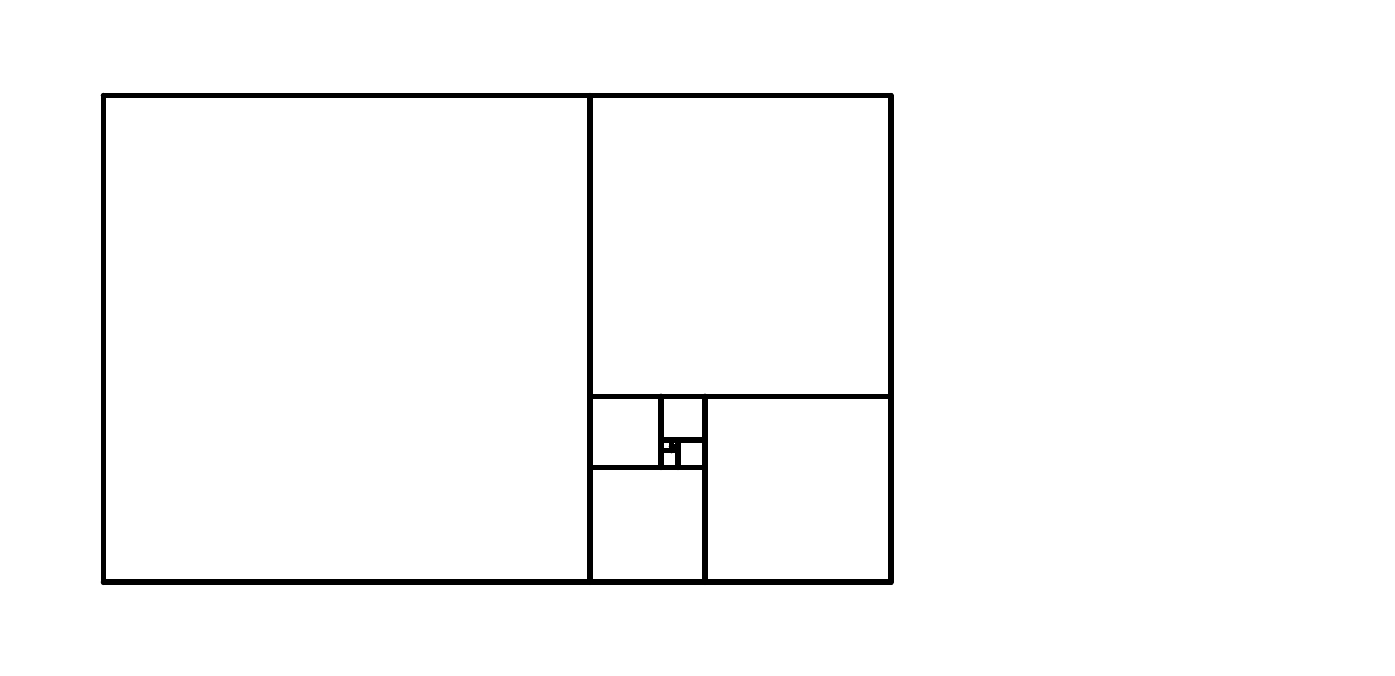
\begin{tikzpicture}[myscale/.style={scale=#1, node distance=#1*10em},myscale=10, line cap=round,line join=round,>=triangle 45,x=1cm,y=1cm]
		
		\clip(-0.09627480300402867,-0.08306212045245437) rectangle (1.60396009090303,0.704296385645171);
		\draw [line width=2pt] (0,0.6180339887498949)-- (0,0);
		\draw [line width=2pt] (1,0.6180339887498949)-- (1,0);
		\draw [line width=2pt] (0,0.6180339887498949)-- (1,0.6180339887498949);
		\draw [line width=2pt] (0.6180339887498949,0.6180339887498949)-- (0.6180339887498949,0);
		\draw [line width=2pt] (0.6180339887498949,0)-- (1,0);
		\draw [line width=2pt] (0.6180339887498949,0)-- (0,0);
		\draw [line width=2pt] (0.6180339887498949,0.23606797749978983)-- (1,0.23606797749978983);
		\draw [line width=2pt] (0.7639320225002102,0)-- (0.7639320225002101,0.23606797749978986);
		\draw [line width=2pt] (0.6180339887498949,0.14589803375031535)-- (0.7639320225002101,0.14589803375031535);
		\draw [line width=2pt] (0.7082039324993696,0.14589803375031532)-- (0.7082039324993699,0.23606797749978986);
		\draw [line width=2pt] (0.7082039324993697,0.18033988749894897)-- (0.7639320225002101,0.18033988749895025);
		\draw [line width=2pt] (0.7294901687515735,0.1803398874989493)-- (0.7294901687515764,0.14589803375031532);
		\draw [line width=2pt] (0.7082039324993697,0.16718427000252123)-- (0.7294901687515744,0.16718427000251893);
		\draw [line width=2pt] (0.7213595499957988,0.1803398874989491)-- (0.7213595499957952,0.16718427000251998);
		\draw [line width=2pt] (0.7213595499957969,0.17220926874317108)-- (0.7294901687515739,0.17220926874316894);
	\end{tikzpicture}

	In den vergangenen Rechtecken wurde fortlaufend das Quadrat so geteilt, das immer ein neues Quadrat entsteht und ein Restrechteck. Diese Schnittstelle teilt immer in den Punkt, welcher den goldenen Schnitt darstellt, da die Länge des Radius des Kreises $l$ ist. Somit ist die Länge der kleineren Seite des Rechtecks und die Seitenlänge des dazugehörigen Quadrats immer zusammen addiert die Länge des vorherigen Quadrats.
\end{document}
